\section{Comparison of FSL FIX and Standard Preprocessing}\label{sec:comp}

The following section will present the results using both the standard preprocessing pipeline and FSL FIX pipeline. First, the signal of brain activation related to the 48$^\circ$ stimulus, achieved from using both methods is presented. Secondly, the difference in the amount of activation achieved by using FSL FIX compared to standard preprocessing will be presented. \\
As mentioned in \secref{sec:stats}, a within heat run, within participant and within group analysis were run on the preprocessed fMRI data. \Figref{fig:res:stdpos} and \figref{fig:res:stdneg} show the intensity of activation and the localization of the positive and negative activation achieved using the standard preprocessing pipeline.  


\begin{figure}[H]                 
	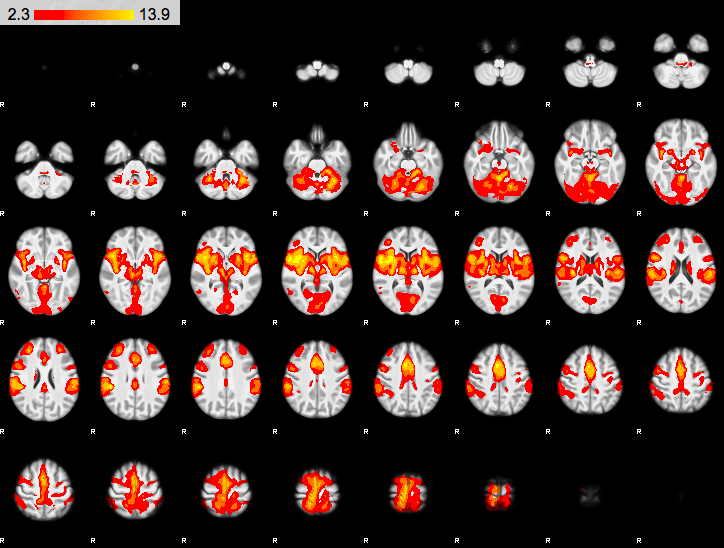
\includegraphics[width=.65\textwidth]{figures/Results/STD_pos}  
	\caption{Results of the achieved positive brain activation after using standard preprocessing with a Z-score range of 2.3 to 13.9. The activation is mainly localized in the regions of the insular cortex, basal ganglia, anterior cingulate cortex, and sensorimotor cortex.}
	\label{fig:res:stdpos} 
\end{figure}

\begin{figure}[H]                 
	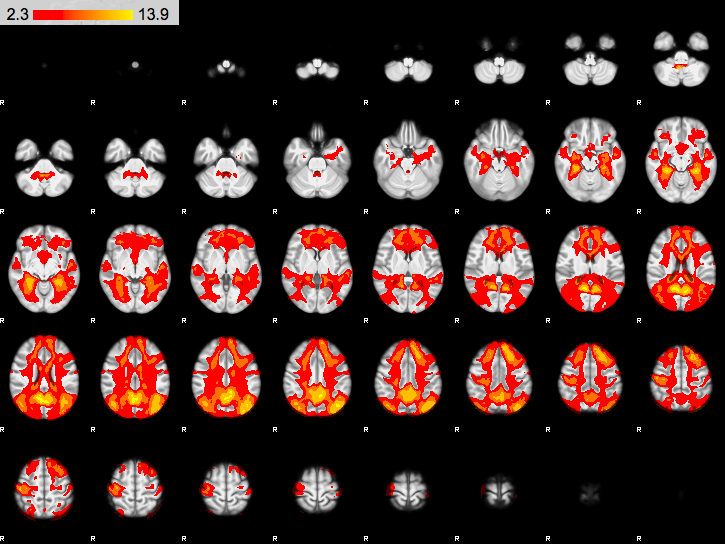
\includegraphics[width=.65\textwidth]{figures/Results/STD_neg}  
	\caption{Results of the achieved negative brain activation after using standard preprocessing with a Z-score range of 2.3 to 13.9. The negative activation is mainly localized in the white matter and the default mode network (prefontal cortex and posterior cingulate cortex).}
	\label{fig:res:stdneg} 
\end{figure}

The localization of regions which are activated during the noxious heat stimuli are primarily those associated with noxious stimuli as presented in \secref{sec:pain}. The main activation is localized in the regions of the insular cortex, basal ganglia, anterior cingulate cortex, and sensorimotor cortex. %The Z-score range of the map has a range 2.3 to 13.9. \\
\Figref{fig:res:FIXpos} and \figref{fig:res:FIXneg} show the intensity of activation and localization of the positive and  negative activation achieved using the FSL FIX preprocessing pipeline. 

\begin{figure}[H]                 
	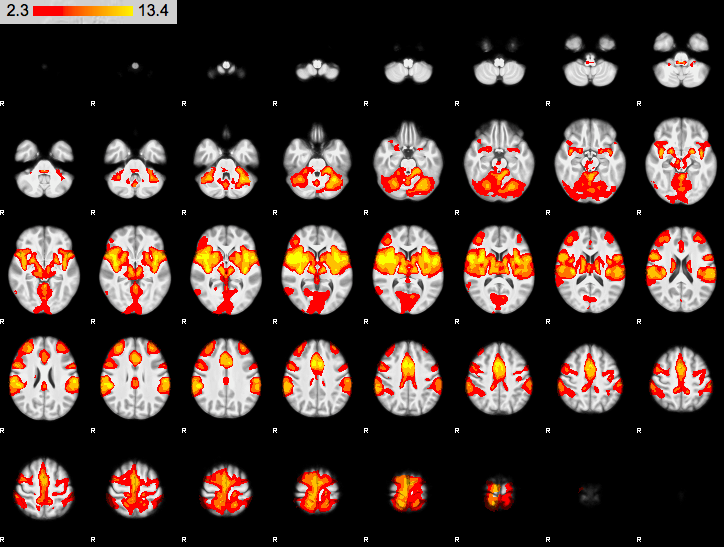
\includegraphics[width=.65\textwidth]{figures/Results/FIX_pos}  
	\caption{Results of the achieved positive brain activation after FIX preprocessing with a Z-score range of 2.3 to 13.4. The activation is mainly localized in the regions of the insular cortex, basal ganglia, anterior cingulate cortex, and sensorimotor cortex.}
	\label{fig:res:FIXpos} 
\end{figure}

\begin{figure}[H]                 
	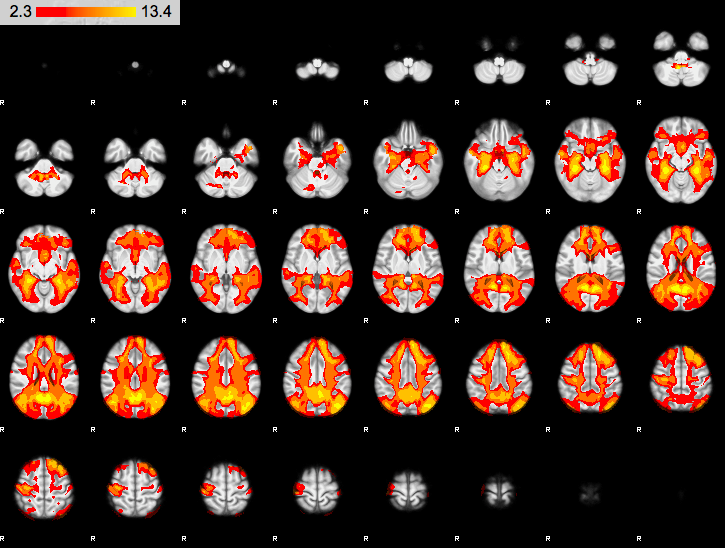
\includegraphics[width=.65\textwidth]{figures/Results/FIX_neg}  
	\caption{Results of the achieved negative brain activation after FIX preprocessing with a Z-score range of 2.3 to 13.4. The negative activation is mainly localized in the white matter and the default mode network.}
	\label{fig:res:FIXneg} 
\end{figure}

The localization and intensity of the activation found by using FIX is very similar to the one seen using standard preprocessing. %The Z-score range is though a bit less as it ranges from 2.3 to 13.4.
The results of using the standard preprocessing pipeline and FSL FIX pipelineare very similar for both the positive and negative activation maps.   
To get statistical measure of the difference in localization and intensity between the two preprocessing methods a comparison was made. The results of this comparison is seen in \figref{fig:res:diff_pos} and \figref{fig:res:diff_neg}. \figref{fig:res:diff_pos} shows where activation is greater for the FIX preprocessed data compared to the standard preprocessed data, and \figref{fig:res:diff_neg} shows where activation is greater the standard preprocessed data compared to the FIX preprocessed data.

\begin{figure}[H]                 
	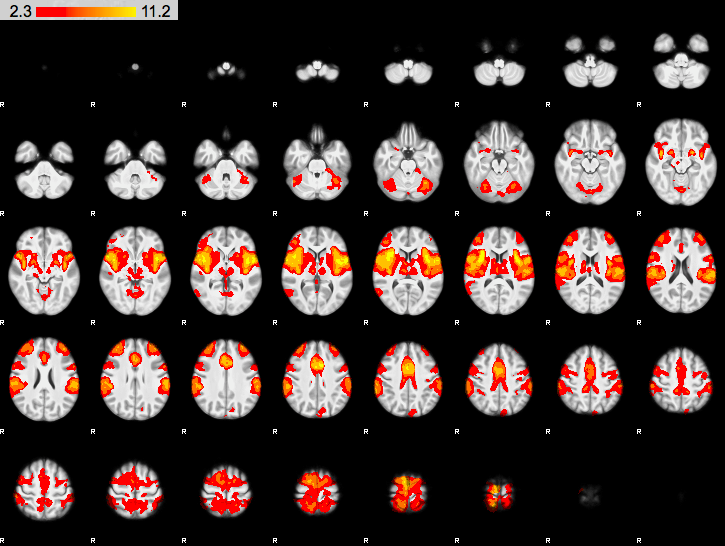
\includegraphics[width=.65\textwidth]{figures/Results/diff_pos}  
	\caption{Results from the comparison of the two preprocessing methods for noise removal. The activation seen is the activation gained with using FIX compared to using standard preprocessing with a Z-score range of 2.3 to 12.1. Increased signal is mainly seen in the insular cortex, anterior cingulate cortex and basal ganglia.}
	\label{fig:res:diff_pos} 
\end{figure}

\begin{figure}[H]                 
	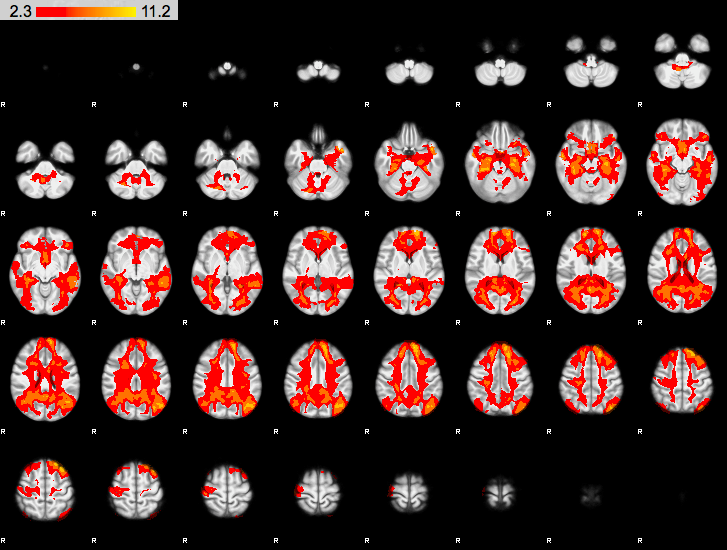
\includegraphics[width=.65\textwidth]{figures/Results/diff_neg}  
	\caption{Results from the comparison of the two preprocessing methods for noise removal. The activation seen in the image is the amount of activation which have been removed by using FIX compared to standard preprocessing with a Z-score range of 2.3 to 11.2. Areas where activation have been removed are white matter and default mode network.}
	\label{fig:res:diff_neg} 
\end{figure}

To summarize the results of using FSL FIX compared to solely using standard preprocessing, FSL FIX does achieve a larger amount of signal related to the noxious stimuli, thereby preserving more signal of interest. Thereby more signal of non interest has been removed using FIX compared to standard preprocessing. 
